\documentclass{acm_proc_article-sp}
\usepackage[utf8]{inputenc}
\usepackage[ngerman]{babel}
\usepackage[backend=bibtex,urldate=long]{biblatex}
\usepackage{color}
\usepackage{float}
\usepackage{graphicx}
\addbibresource{lit.bib}

\begin{document}
\title{Feststellung und Bewertung des Melodie- und Rhythmusgedächtnisses}
\subtitle{Lehrgebiet Audiotechnik SS2015 31.07.2015}
%\subtitle{Lehrverantwortliche: Dr. rer. nat. Dieter Kemter, PD Dr.-Ing. habil. Günther Schatter }

\numberofauthors{2} 
\author{
% 1st. author
\alignauthor
Kristof Komlossy\\
       \affaddr{Bauhaus-Universität Weimar}\\
       \affaddr{Fakultät Medien}\\
       \email{kristof.komlossy@uni-weimar.de}
% 2nd. author
\alignauthor
Jakob Harlan\\
       \affaddr{Bauhaus-Universität Weimar}\\
       \affaddr{Fakultät Medien}\\
       \email{jakob.harlan@uni-weimar.de}
} %author

\maketitle

\begin{abstract}
In dieser Arbeit wird untersucht, ob das Kurzzeitgedächtnis unterschiedliche Leistungen beim Rekapitulieren von Melodien und Rhythmen aufweist. Dazu haben wir Programme zum Testen des Melodiegedächtnisses und des Rhythmusgedächtnisses entwickelt und in einer Nutzerstudie eingesetzt. Die Programme und die Ergebnisse der Nutzerstudie werden wir in der vorliegenden Arbeit vorstellen und auswerten.
\end{abstract}

\keywords{Rhytmusgedächtnis, Melodiegedächtnis, Max\slash MSP} % NOT required for Proceedings

\section{Einleitung}
Wir haben uns mit der Fragestellung beschäftigt, ob das Kurzzeitgedächtnis unterschiedliche Leistungen beim Rekapitulieren von Melodien und Rhythmen aufweist. Um diese Frage zu beantworten haben wir uns dazu entschieden mit musikalischen Tests das Gedächtnis von Personen zu überprüfen und zu analysieren.\\
Zu Beginn (2) werden wir die bereits existierenden und für uns relevanten musikalischen Tests vorstellen.\\
Auf diese bereits vorhandenen Untersuchungen haben wir unsere Vorüberlegungen aufgebaut (3) und haben je ein Programm zum Testen von zwei ähnlichen musikalischen Fähigkeiten entwickelt. Zum einen haben wir ein Programm zum Testen des Melodiegedächtnisses entwickelt. Dieses Programm spielt dem Nutzer eine Melodie vor. Anschließend muss der Nutzer die Melodie aus dem Gedächtnis rekapitulieren können und dabei die relativen Tonhöhen bestimmen können.\\
Die zweite Fähigkeit die wir getestet haben ist das Rhythmusgedächtnis. Ähnlich wie bei dem Melodiegedächtnis spielt das Programm dem Nutzer einen Rhythmus vor, welchen der Nutzer dann ebenfalls aus dem Gedächtnis wiedergeben muss. Da die Rhythmen aus drei verschiedenen Tonlängen zusammengesetzt sind muss der Nutzer angeben welche Länge jeder einzelne Ton hatte. Auf die nähere Implementierung dieser Programme werden wir in Kapitel 4 eingehen.\\
Um unsere zu Beginn genannten Fragestellungen zu beantworten haben wir mit unseren beiden Programmen eine Nutzerstudie durchgeführt. Die Beschreibung der Studie und die Auswertung der Ergebnisse werden wir in Kapitel 5 vornehmen.

\section{Verwandte Arbeiten}
Im Jahr 1919 hat der amerikanische Psychologe Carl Emil Seashore eine Reihe von Tests zur Ermittlung musikalischer Begabung entwickelt\cite{gordon:2000}. Seashore hat für diese Arbeit fast 20 Jahre das Thema der Charakterisierung und Beschreibung musikalischer Begabung untersucht. Das Ergebnis waren erstmalig standardisierte Tests zur Ermittlung musikalischer Fähigkeiten. Dabei fokussierte sich Seashore auf das Gedächtnis für Ton- und Rhythmusfolgen und die Unterscheidungsfähigkeit folgender Eigenschaften: Tonhöhen, Lautstärken, Rhythmen, Tonlängen, und Klangfarben.
Aufgrund des hohen Grades der Standardisierung der Seashore-Tests und der grundlegenden Forschung vor Ihrer Entwicklung wurden die Tests häufig von anderen musikalischen Tests als Grundlage genutzt.

Einer dieser Tests, welcher den Seashore-Test als Grundlage genutzt hat ist der "`Wiener Test für Musikalität"'\cite{laengle:2003}. Dieser Test entstand im Februar 2003 in Zusammenarbeit diverser Psychologen und Pädagogen unter anderem der Universität Wien. Der Test war der erste computerbasierte Musikbegabungstest und richtete sich an Vor- oder Grundschulkinder. Der "`Wiener Test für Musikalität"' greift zwei von dem Seashore-Test untersuchte musikalische Fähigkeiten auf: Zum einen wird die Fähigkeit der Wahrnehmung von Rhythmusschwankungen der Kinder geprüft. Dazu werden drei Töne vorgespielt, wobei der erste und der letzte Ton im Takt gespielt werden. Der Ton in der Mitte wird manchmal leicht versetzt zum eigentlichen zweiten Schlag gespielt. Der Test besteht darin, anzugeben ob der zweite Ton vorgezogen, auf den Schlag genau oder etwas zu spät gespielt wird.\\
Der zweite Teil des Tests untersucht die Fähigkeit Änderungen in der Tonhöhe zweier Töne zu unterscheiden. Dazu wird ein Zweiklang vorgespielt und man muss angeben welcher der drei Fälle eintritt: Im ersten Fall gleitet einer der Töne etwas nach oben und wieder zurück, im zweiten Fall gleitet einer der Töne etwas nach unten und im dritten Fall verändert sich keiner der Töne. In diesem Test wurden die beiden zeitgleich gespielten Töne als Delfine dargestellt (Abbildung~\ref{pic:wienertest}). Die Kinder müssen angeben, ob einer der Delfine nach oben, nach unten oder auf der gleichen Höhe relativ zum anderen Delfin geschwommen ist. 
\begin{figure}[H]
\centering
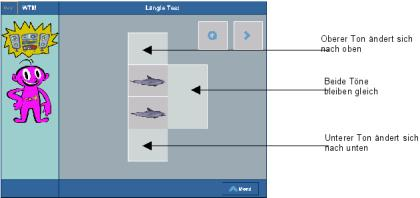
\includegraphics[width=1.0\linewidth]{Abbildungen/wienertest.jpg}
\caption{Wiener Test für Musikalität}
\label{pic:wienertest}
\end{figure}

\section{Konzept}
Um eine Software zum Erkennen musikalischer Fähigkeiten umzusetzen haben wir uns an dem "`Wiener Test für Musikalität"' orientiert.
Die Grund für diese Wahl war unsere Absicht eine Nutzerstudie durchzuführen. Für eine sinnvolle und zielführende Konzeptionierung dieser Nutzerstudie sollten die Anzahl der Tests überschaubar sein und die Tests untereinander vergleichbar sein.
Daher haben wir haben die Tests zur Tonhöhen- und Rhythmusänderungswahrnehmung als Grundlage genommen und um den Aspekt des Erinnerns von Tonfolgen erweitert.
Um die Vergleichbarkeit der Tests weiter zu erhöhen haben wir auch den Ablauf und die Bedienung der Tests ähnlich gestaltet.
Zu Beginn kann sich eine Melodie beziehungsweise ein Rhythmus einmal oder bei Bedarf mehrfach angehört werden. Anschließend "'startet"' man per Knopfdruck den eigentlichen Test. Die zuvor angehörte Tonfolge kann nun nicht mehr wiederholt werden. Die Rekapitulation der Tonfolgen unterscheidet sich leicht bei dem Rhythmus- beziehungsweise Melodietest. Bei dem Rhythmustest muss man die Länge jedes Tones der Tonfolge angeben. Die Rhythmen sind aus Tönen mit insgesamt drei verschiedenen Tonlängen zusammengesetzt. Man muss also für jeden Ton angeben ob er kurz, mittel oder lang ist. Den Ton mittlerer Länge kann man sich auch nach dem Starten des Tests noch anhören um eine Referenz zu erhalten.\\
Bei dem Melodietest kann man sich den ersten Ton der Tonfolge anhören. Anschließend muss man, beginnend bei dem Zweiten für jeden Ton angeben, ob der aktuell betrachtete Ton relativ zum vorherigen Ton höher, gleich oder tiefer in der Tonhöhe liegt.\\ 
Im Gegensatz zum "`Wiener Test für Musikalität"' wollten wir nicht die Fähigkeit die Änderungen in Tonlänge und Tonhöhe zu erkennen testen sondern wie gut diese gemerkt werden können. Deswegen unterscheiden sich sowohl die Tonlängen im Rhythmustest als auch die Tonhöhen im Melodietest klar.

\section{Implementierung}
Die beiden Programme haben wir mit der grafischen Entwicklungsumgebung und visuellen Programmiersprache Max\slash MSP\footnote{https://cycling74.com/products/max/} implementiert. Die erste Version von Max\slash MSP (MSP steht für Max Signal Processing) \cite{wiki:max} wurde 1988 entwickelt und wird seitdem von Komponisten, Musikern und Künstlern eingesetzt um interaktive Programme zu entwickeln. Da Max\slash MSP eine grafische Programmiersprache und zusätzlich auf audiobezogene Software ausgelegt ist eignet sich die Sprache für einen Test zur Feststellung musikalischer Fähigkeiten.\\
Eine grafische Oberfläche ist durch die vorgegebenen Objekte, von denen einige unter anderem aus Knöpfen, Schiebereglern, Optionsschaltflächen oder Kombinationen aus diesen bestehen, schnell und mit geringem Aufwand umzusetzen. Durch diese Eingabeobjekte erfolgt auch die Interaktion mit dem Testprogramm. In Abbildung~\ref{maxfirststep} ist die Interaktionsoberfläche unseres Melodieprogramms dargestellt. Neben einem Feld für die Teilnehmernummer für die Studie haben wir in der obersten Reihe drei Knöpfe. Der erste erstellt einen neuen Nutzer, der zweite erstellt einen neuen Test und der letzte startet den Test der aktuellen Tonfolge.
Unter den Knöpfen befindet sich eine Optionsschaltfläche zum Auswählen der zu Testenden Tonfolge. Diese kann sich mit dem "'play~melody"'-Knopf angehört werden.\\
Drückt man auf "'start~test"' geht die Oberfläche in den zweiten Präsentationsstatus über (Abbildung~\ref{maxfirststep}). Dort kann man sich im Fall des Melodiegedächtnistests den erste Ton der Folge noch einmal anhören ("play~first~note"). Die Eingabe der erinnerten Tonfolgen erfolgt dann über die in der letzten Zeile angezeigten Optionsschaltflächen. Möchte man das eingegebene Ergebnis speichern drückt man auf den "'save~input"'-Knopf. 

\begin{figure}[H]
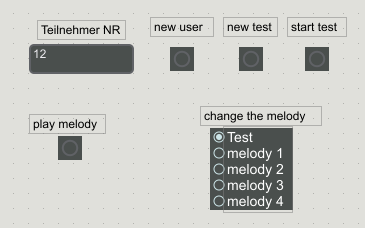
\includegraphics[width=1.0\linewidth]{Abbildungen/firststep.png}
\caption{Oberfläche zum Anhören der Tonfolgen}
\label{maxfirststep}
\end{figure}

\begin{figure}[H]
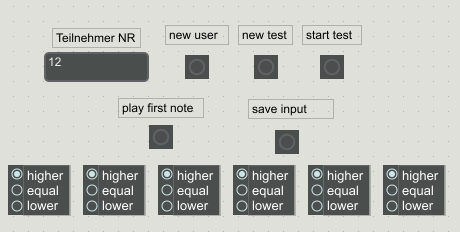
\includegraphics[width=1.0\linewidth]{Abbildungen/secondstep.png}
\caption{Oberfläche zum Rekapitulieren der Tonfolgen}
\label{maxsecondstep}
\end{figure}

Die Tonfolgen werden über das MIDI-Interface von Max an die Soundkarte des Computer weitergegeben um für den Nutzer hörbar gemacht zu werden. Mit dem "'makenote"'-Objekt\footnote{https://docs.cycling74.com/max5/refpages/max-ref/makenote.html} von Max\slash MSP werden MIDI-Befehle erzeugt. Als Eingabe-Parameter des Objektes haben wir die Tonhöhe des aktuellen Tones, die Anschlagsstärke und die Dauer des Tones  eingegeben. Das Objekt gibt daraufhin die Tonhöhe als Zahl gepaart mit der Anschlagstärke aus (note-on-Befehl). Nachdem die als Eingabe-Parameter übergebene Länge des Tones zeitlich verstrichen ist, sendet das Objekt erneut die Tonhöhe als Ausgabe aus, dieses Mal jedoch gepaart mit der Anschlagstärke 0 (note-off-Befehl).\\
Die Ausgaben des "'makenote"'-Objektes gehen direkt in das "'noteout"'-Objekt\footnote{https://docs.cycling74.com/max5/refpages/max-ref/noteout.html}. Dieses nimmt die Eingabe-Parameter und sendet die note-on- und note-of-Befehle an den MIDI-Port. Als zusätzlichen Eingabe-Parameter kann man bei dem "'noteout"'-Objekt den MIDI-Kanal wählen. Da wir jedoch nur Klaviertöne benötigen haben wir die Standardeinstellungen, Kanal 1, übernommen.

In Abbildung~\ref{pic:max} sieht man einen Ausschnitt aus unseren Programmen. Die Melodie, dargestellt als Felder mit den der Tonhöhe entsprechenden Zahlen enthaltend wird vor Kontakt mit dem "'makenote"'-Objekt gefiltert. Wird ein Ton mit Tonhöhe 0 abgespielt, wird dieser Ton als Pause gewertet und wird rausgefiltert und das "'makenote"'-Objekt wird nicht aktiviert. Alle anderen Töne gelangen als erstes Argument in das "'makenote"'-Objekt. Dieses erhält zwei weitere Argumente: Das zweite Argument bestimmt die Anschlagsstärke, das dritte Argument die Länge des Tones. Auf der Abbildung ist zu erkennen, dass wir 127 als Standardanschlagsstärke und 200 als Standardtonlänge gewählt haben.\\
Die beiden vom "'makenote"'-Objekt abgehenden Verbindungen führen direkt in das "'noteout"'-Objekt. Über die erste Verbindung wird die Tonhöhe und über die zweite Verbindung wird die Anschlagsstärke des Tones übermittelt. Das "'noteout"'-Objekt besitzt einen dritten Verbindungsanschluss über den der MIDI-Kanal gewählt wird. Wie oben beschrieben haben wir dort die Standardeinstellung belassen.
\begin{figure}[H]
\centering
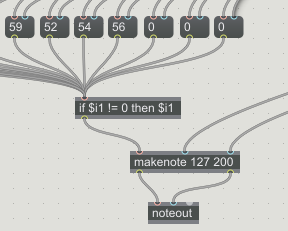
\includegraphics[width=1.0\linewidth]{Abbildungen/max.png}
\caption{Ausschnitt aus unseren Programmen: Wiedergabe von Töne mit dem "'makenote"'- und "'noteout"'-Objekt}
\label{pic:max}
\end{figure}

\section{Studie}
In diesem Kapitel wird die Konzeption, Durchführung, Beobachtung, qualitative und statistische Auswertung der von uns durchgeführten Studie vorgestellt. Zuletzt werden die Vorgehensweisen und Ergebnisse diskutiert.

\subsection{Design \& Fragestellungen}
In unserer Studie sollte von möglichst vielen Testpersonen sowohl das Melodie- als auch das Rhythmusgedächtnis getestet werden. Dafür haben wir die von uns entwickelten Programme verwendet.\\
Außerdem sollte die Studie Auskunft darüber geben welche Faktoren zu einer guten Leistung in den getesteten Bereichen führt. Hierfür erhoben wir folgende Informationen über die Teilnehmer:
\begin{itemize} 
\item Alter
\item Geschlecht
\item Musikalische Vorkenntnisse
\item Antworten des Testes
\item Abspielanzahl der einzelnen Samples
\item Empfundene Schwierigkeit bei beiden Tests
\end{itemize}
Unsere zentrale Hypothese ist, dass musikalische Vorkenntnisse hilfreich bei der Bewältigung der Aufgaben sind. Diese galt es zu validieren.\\
Auch ob Alter oder Geschlecht einen messbaren Unterschied machen interessierte uns. Ebenfalls haben wir untersucht ob die empfundene Schwierigkeit mit dem tatsächlichen Ergebnis der Kandidaten korreliert.\\ 
Unterschiede zwischen den beiden Tests wollten wir auch analysieren. Also ob es gleich schwer ist sich Rhythmen oder Melodien zu merken. Und auch ob Personen immer in beiden Tests ähnlich abschneiden oder es Personen gibt denen eine Aufgabe deutlich leichter fällt.
% War der 2te Test erfolgreicher?
\subsection{Durchführung}

\subsubsection{Ablauf}
Um die nötigen Informationen zu erheben musste vor dem eigentlichen Test ein Fragebogen beantwortet werden, welcher Alter, Geschlecht und musikalische Vorkenntnisse abfragt. Die musikalischen Vorkenntnisse haben die Kandidaten auf einer Skala von 1-10 selber bewertet. Allerdings haben hier die begleitenden Studienautoren beratend eingegriffen um Vergleichbarkeit zu gewährleisten.\\
Darauf folgend wurde der Testperson die Programmoberfläche und der Ablauf der Tests erklärt.\\ 
Die Kandidaten mussten jeweils eine Testreihe zum Rhythmusgedächtnis und eine zum Melodiegedächnis absolvieren. Die Reihenfolge wurde zwischen den Teilnehmern alternierend gewählt um Lerneffekte auszuschließen. \\

Bei beiden Testreihen gibt es fünf verschiedene Tonfolgen. Jede besteht aus sechs bis elf einzelnen Tönen. Die erste Tonfolge ist bei beiden Tests als Vorbereitung gedacht. Diese sind möglichst einfach gewählt: Eine bekannte Melodie (Jingle Bells) und eine einfache Rhythmusfolge. Durch diese Beispiele wird der Kandidat mit dem Ablauf, der Programmbedienung und der Antwortform bekannt gemacht. Die Resultate hiervon wurden nicht in die Auswertung übernommen. \\
Die übrigen vier Rhythmusfolgen waren Eigenkompositionen mit höherer Komplexität als der Einstiegsrhythmus.
Drei unserer vier übrigen Melodiefolgen waren Teile einer Melodie für unsere Nutzer möglichst unbekannter Musikstücke.
Zwei dieser Melodien stammen aus dem Lied "`The Darkest Nights"' der Band "`As I Lay Dying"', die dritte Melodie stammt aus einer Komposition von Bach.\\
Die fünfte Melodie ist eine selbst komponierte Tonfolge. Durch diese Diversität der Melodien erhoffen wir uns repräsentative Ergebnisse für das Melodiegedächtnis \textcolor{red}{<- dann eigentlich auch bei den rhythmen, da aber alles eigenkomposition}. Die Tonfolgen dürfen beliebig häufig angehört werden, bevor der Teilnehmer die Antworten gibt.
 
Nach den Tests mussten die Kandidaten noch einen weiteren kurzen Fragebogen ausfüllen in dem aufgenommen wurde wie schwer sie die einzelnen Tests gefunden haben. Außerdem stand hier ein Textfeld für freie Kommentare zur Verfügung. 

\subsubsection{Teilnehmer}
Die Studie wurde mit 23 Teilnehmern durchgeführt.\\
Die meisten wurden aus unserem studentischen Umfeld akquiriert, was die unrepräsentative Altersverteilung (Abbildung \ref{Alter}), mit einer deutlichen Häufung im Bereich 20-25 Jahre, erklärt. Die davon abweichenden Kandidaten sind Familienmitglieder und andere Bekannte.
\begin{figure}[h]
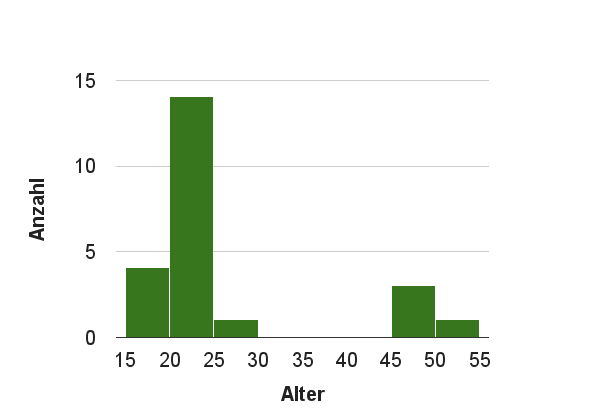
\includegraphics[width=1.0\linewidth]{Abbildungen/Altersverteilung.png}
\caption{Altersverteilung}
\label{Alter}
\end{figure}
Ungefähr die Hälfte der Teilnehmer stammt aus dem Bereich der Informatik. Die anderen verteilen sich auf weitere Studienfächer, Schüler und Berufstätige.\\
Es ist uns gelungen gleichmäßig viele weibliche und männliche Teilnehmer zu testen (11 Weibliche und 12 Männliche). 
\subsection{Auswertung}
Als Maß für den Erfolg diente die relative Erfolgshäufigkeit. Hierbei wurden die Anzahl richtig beantworteten Töne durch die Anzahl aller Töne geteilt. So sind alle Töne gleich gewichtet. Die Länge der einzelnen Tonfolgen hat keinen Einfluss.
\subsubsection{Statistische Auswertung}
Insgesamt waren 72,3\% der Antworten richtig. Wobei Melodien etwas besser wiedergegeben wurden (73,6\%) als Rhythmen (71,0\%). Abbildung \ref{MelodieGegenRhythmus} zeigt dass generell Testpersonen mit guten Leistungen im Melodietest auch im Rhythmustest erfolgreich waren und umgekehrt.
\begin{figure}[H]
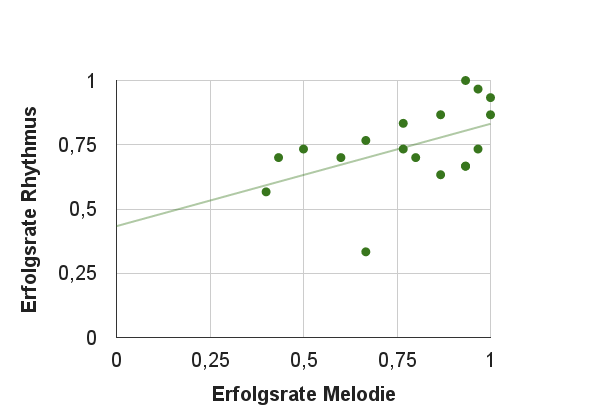
\includegraphics[width=1.0\linewidth]{Abbildungen/Melodie-Rhythmus.png}
\caption{Melodie gegen Rhythmus}
\label{MelodieGegenRhythmus}
\end{figure}
Der visuelle Eindruck eines Zusammenhangs wird vom linearen Korrelationskoeffizient nach Pearsons \cite{wiki:korrelationskoeffizient} (0,59) unterstützt. Und auch der Rangkorrelationskoeffizient nach Spearman \cite{wiki:rangkorrelationskoeffizient} (0,60) widerspricht diesem nicht.\\

Die von uns aufgestellte Hypothese, dass musikalische Vorkenntnisse das Melodie- und Rhythmusgedächnis stärken wird von den Ergebnissen unserer Studie bestätigt. Abbildung \ref{ErfolgGegenVorkenntnisse} zeigt genau diesen Zusammenhang.
%http://www.socscistatistics.com/tests/spearman/Default2.aspx
\begin{figure}[H]
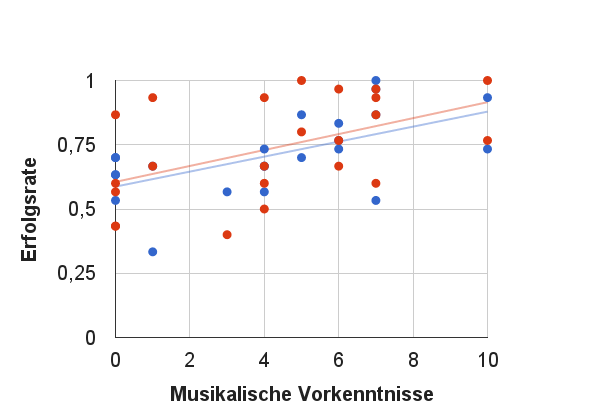
\includegraphics[width=1.0\linewidth]{Abbildungen/Einschaetzung-Melodie_Rhythmus.png}
\caption{Erfolgsraten gegen Vorkenntnisse (Melodie Rot, Rhythmus Blau)}
\label{ErfolgGegenVorkenntnisse}
\end{figure}
Die Korrelationskoeffizienten belegen dies (Pearson: 0.50 für Melodie, 0.59 für Rhythmus. Spearman: 0.54 für Melodie, 0.65 für Rhythmus).\\\\

Eine Zusammenhang zwischen Alter oder Geschlecht und der erbrachten Leistung konnte nicht gefunden werden. In Abbildung \ref{Geschlechter} sieht man das die Ergebnisse zwischen den Geschlechtern nahezu identisch sind (Unterschied: 0.8\%). \\
\begin{figure}[H]
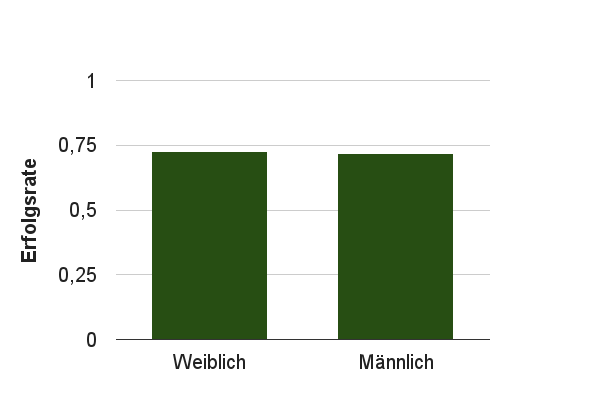
\includegraphics[width=1.0\linewidth]{Abbildungen/Geschlecht-Erfolg.png}
\caption{Erfolgsraten der Geschlechter}
\label{Geschlechter}
\end{figure}
Die empfundene Schwierigkeit der Aufgaben hängt, wie zu erwarten war,  mit den tatsächlichen Ergebnissen zusammen. Zu Sehen sind diese Zusammenhänge in Abbildung \ref{EmpfindungMelodie} und \ref{EmpfindungRhythmus}.
\begin{figure}[H]
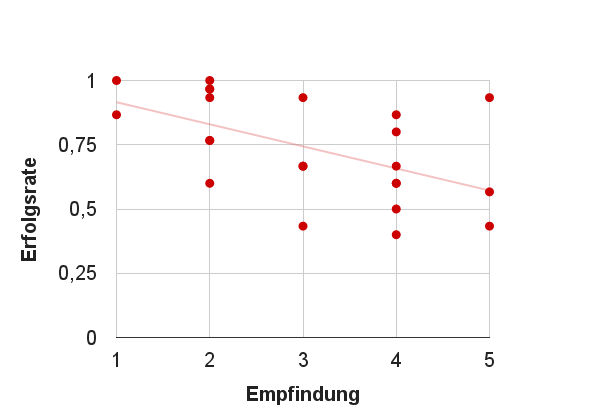
\includegraphics[width=1.0\linewidth]{Abbildungen/Empfindung-Erfolg_Melodie.png}
\caption{Empfindung gegen Erfolg - Melodie}
\label{EmpfindungMelodie}
\end{figure}
\begin{figure}[H]
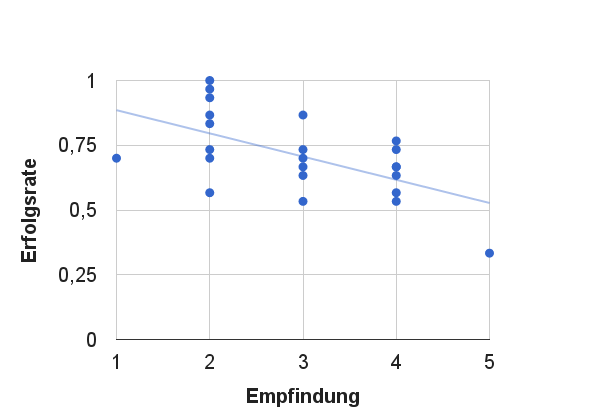
\includegraphics[width=1.0\linewidth]{Abbildungen/Empfindugn-Erfolg_Rhythmus.png}
\caption{Empfindung gegen Erfolg - Rhythmus}
\label{EmpfindungRhythmus}
\end{figure}
Allgemein gilt, dass umso schwerer die Aufgabe empfunden wurde desto schlechter waren die erbrachten Leistungen. Die negativen Korrelationskoeffizienten zeigen dies (Pearson: -0.54 für Melodie, -0.59 für Rhythmus. Spearman: -0.57 für Melodie, -0.54 für Rhythmus).

Während der Durchführung der Studie ist uns aufgefallen das scheinbar viele Kandidaten besonders Probleme damit hatten die langen Töne korrekt zu erkennen. Also haben wir ausgewertet wie gut die einzelnen Längen der Rhythmus-Tonfolgen wiedergegeben wurden (Abbildung \ref{Tonlängen}). Und ob Unterschiede in der Erfolgshäufigkeit zwischen höheren, gleichen und niedrigeren Tönen des Melodietestes gab (Abbildung \ref{Tonhöhen}).
\begin{figure}[H]
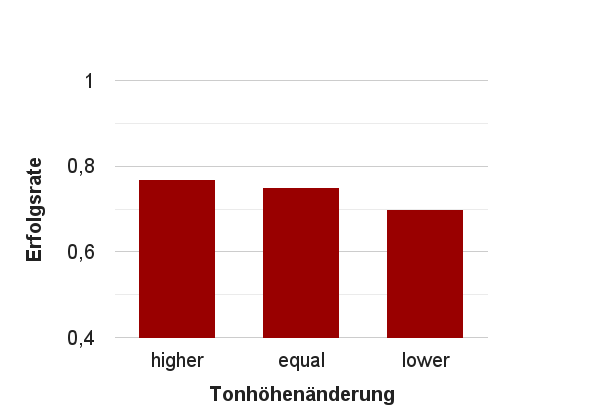
\includegraphics[width=1.0\linewidth]{Abbildungen/Tonhoehenaenderung-Erfolg.png}
\caption{Tonhöhenänderung gegen Erfolg}
\label{Tonhöhen}
\end{figure}
\begin{figure}[H]
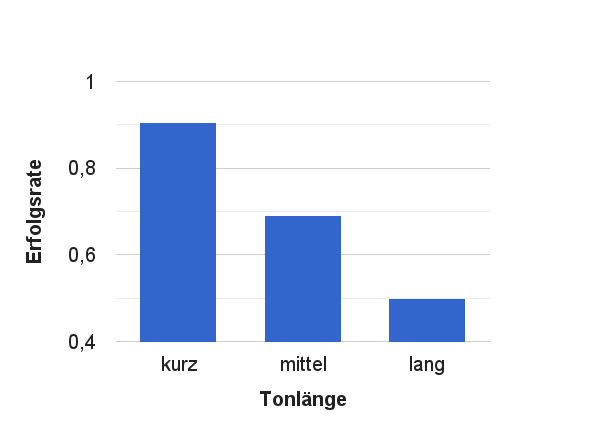
\includegraphics[width=1.0\linewidth]{Abbildungen/Tonlaenge-Erfolg.png}
\caption{Tonlängen gegen Erfolg}
\label{Tonlängen}
\end{figure}
Die Vermutung wurde bestätigt. Die Erfolgsrate der langen Töne ist, mit nur 50\%, deutlich die schlechteste. Die Kurzen dagegen wurden in über 90\% der Fälle erkannt. Beim Melodietest sind keine ähnlich großen Unterschiede aufgetreten. Die verringernden Tonfolgen wurden zwar schlechter wiedergegeben als die anderen Fällen, aber die Unterschiede betragen nur 5-7\%.
\subsubsection{Beobachtungen}
Beim Begleiten der Testpersonen durch die Studie konnten wir noch Interessantes abseits der erhobenen Daten beobachten, worauf hier eingegangen werden soll.\\

Wir haben zwischen den Kandidaten unterschiedliche Vorgehensweisen beim Merken der Tonfolgen erkannt. Insbesondere die Frequenz des Abspielens variierte stark. Es gab Kandidaten die haben sich ein Stück nur zweimal angehört. Zwischen den Abspielungen haben sie versucht sich an das Gehörte zu erinnern und sich selber mental vorzuspielen. Beim zweiten mal haben sie ihre Vorstellung und die Wirklichkeit verglichen. Dies hat ihnen gereicht um sich sicher zu fühlen korrekt antworten zu können.\\
Andere dagegen haben die Beispiele sobald sie endeten wieder abgespielt und keine Pausen entstehen lassen. Dieser Ansatz hat Abspielhäufigkeiten von 10 Wiederholungen und mehr verursacht.\\ 
Was zu diesen unterschiedlichen Ansätzen zum Merken führt und ob diese verschieden gute Ergebnisse erreichen kann mit unserer Studie nicht beantwortet werden.\\

Ein weitere Besonderheit die wir beobachtet haben ist das einige Teilnehmer Probleme hatten die gemerkte Tonfolge in die von uns erwartete Notation zu überführen. Da viele Kandidaten das gemerkte Beispiel summten, konnte der begleitende Experte klar erkennen das es sich korrekt gemerkt wurde. Doch beim Einordnen der Töne in höher, gleich, tiefer beziehungsweise kurz, mittel, lang wurden trotzdem Fehler gemacht.
\subsection{\textcolor{green}{Diskussion}}
Die erzielten Ergebnisse sind mit gewisser Vorsicht zu betrachten. Uns sind während und nach der Studie Kritikpunkte aufgefallen die die Aussagekraft gegebenenfalls abschwächen.\\
Wir hatten zu wenig Teilnehmer und diese waren auch nicht ausreichend repräsentativ verteilt. Wir hätten uns entweder für einen Test nur innerhalb einer kleineren Zielgruppe entscheiden können. Zum Beispiel Studierende. Oder wir hätten repräsentative Stichprobe der Bevölkerung gebraucht was natürlich einen erheblichen Mehraufwand bedeutet.\\
Auch das Nutzen von festgelegten Rhythmen und Melodien könnte verzerrte Ergebnisse produziert haben. Für bestimmte Zielsetzungen hätten zufällig generierte Beispiele sichere Resultate hervorgebracht.\\
Das Problem, dass Kandidaten trotzt korrektem Gedächtnis nicht in der Lage waren fehlerfrei zu antworten zeigt Verbesserungspotential an den gewählten Antwortsystemen. Wenn, wie hier, nur die Gedächtnisleistung getestet werden soll muss ein Weg gefunden werden das solche Fehler nicht auftreten. Dies könnte durch ein intuitiveres System oder eine ausführlichere Einführung erreicht werden.\\

\subsubsection{Schlussfolgerungen}
Die gesammelten Informationen müssen mit den Rahmenbedingungen und den Schwierigkeiten der Studie in Bezug gesetzt werden um Schlussfolgerungen ziehen zu können.

Das musikalische Vorkenntnisse und Erfahrungen bei der Bearbeitung der Aufgaben Vorteile bringen lies sich bestätigen. Doch wie genau diese Vorteile aussehen konnte nicht beantwortet werden. Ob Personen mit Vorkenntnissen sich tatsächlich die Tonfolgen besser merken konnten, oder einfach der häufige Umgang mit Tönen, Noten und Rhythmen das Übersetzten in unsere Antwortform erleichtert hat ist nicht klar zu erkennen.\\
Für die stärker ausgeprägte Korrelation zwischen Vorkenntnissen und Rhythmusgedächnis als zwischen Vorkenntnissen und Melodiegedächnis haben wir zwei mögliche Erklärungen. Zum einen kann es sein, dass das Erkennen,Merken und Wiedergeben von Tonlängen eine anspruchsvollere Tätigkeit ist als von Tonhöhen. Somit haben Vorkenntnisse und Erfahrung einen größeren Einfluss. \\
Eine andere Erklärung könnte sein, dass gerade bei weniger ausgeprägten musikalischen Vorkenntnissen viele Personen im alltäglichen Leben mehr mit Melodien als mit Rhythmen beziehungsweise Tonlängen konfrontiert werden. Dadurch würde auch ohne explizite musikalische Ausbildung oder Erfahrungen das Melodiegedächnis gefördert werden.\\
%Empfindung
%Tonhöhenänderung / Länge

\section{Verbleibende Arbeiten}
Wir haben ein System zur Feststellung und Bewertung des Melodie- und Rhythmusgedächtnisses entwickelt, dieses implementiert und in einer Studie angewandt.  
Wir konnten in unserer Studie einige Ergebnisse sammeln und Fragestellungen beantworten. Noch mehr haben wir allerdings Denkanstöße bekommen und Details aufgedeckt an den man weiter arbeiten könnte.\\
Eine Wiederholung dieser Studie mit einem gleichmäßigeren und größeren Teilnehmerfeld ist sicherlich interessant. Aber auch Fragestellungen danach wie lang eine Tonfolge sein darf um diese im Kurzzeitgedächtnis zu halten und ob Melodien beziehungsweise Rhythmen mit musischer Qualität leichter erinnert werden als Zufallsprodukte würden wir gerne untersuchen.

\section{Danksagungen}
Zuletzt möchten wir den Lehrverantwortlichen Dr. rer. nat. Dieter Kemter und PD Dr.-Ing. habil. Günther Schatter für die Einführung in dieses spannende Lehrgebiet dankten. Besonderer Dank geht an alle freiwilligen Teilnehmer der Studie ohne die diese Arbeit nicht möglich gewesen wäre.

\printbibliography
\end{document}
